\documentclass{beamer}\usepackage[]{graphicx}\usepackage[]{color}
%% maxwidth is the original width if it is less than linewidth
%% otherwise use linewidth (to make sure the graphics do not exceed the margin)
\makeatletter
\def\maxwidth{ %
  \ifdim\Gin@nat@width>\linewidth
    \linewidth
  \else
    \Gin@nat@width
  \fi
}
\makeatother

\definecolor{fgcolor}{rgb}{0.345, 0.345, 0.345}
\newcommand{\hlnum}[1]{\textcolor[rgb]{0.686,0.059,0.569}{#1}}%
\newcommand{\hlstr}[1]{\textcolor[rgb]{0.192,0.494,0.8}{#1}}%
\newcommand{\hlcom}[1]{\textcolor[rgb]{0.678,0.584,0.686}{\textit{#1}}}%
\newcommand{\hlopt}[1]{\textcolor[rgb]{0,0,0}{#1}}%
\newcommand{\hlstd}[1]{\textcolor[rgb]{0.345,0.345,0.345}{#1}}%
\newcommand{\hlkwa}[1]{\textcolor[rgb]{0.161,0.373,0.58}{\textbf{#1}}}%
\newcommand{\hlkwb}[1]{\textcolor[rgb]{0.69,0.353,0.396}{#1}}%
\newcommand{\hlkwc}[1]{\textcolor[rgb]{0.333,0.667,0.333}{#1}}%
\newcommand{\hlkwd}[1]{\textcolor[rgb]{0.737,0.353,0.396}{\textbf{#1}}}%
\let\hlipl\hlkwb

\usepackage{framed}
\makeatletter
\newenvironment{kframe}{%
 \def\at@end@of@kframe{}%
 \ifinner\ifhmode%
  \def\at@end@of@kframe{\end{minipage}}%
  \begin{minipage}{\columnwidth}%
 \fi\fi%
 \def\FrameCommand##1{\hskip\@totalleftmargin \hskip-\fboxsep
 \colorbox{shadecolor}{##1}\hskip-\fboxsep
     % There is no \\@totalrightmargin, so:
     \hskip-\linewidth \hskip-\@totalleftmargin \hskip\columnwidth}%
 \MakeFramed {\advance\hsize-\width
   \@totalleftmargin\z@ \linewidth\hsize
   \@setminipage}}%
 {\par\unskip\endMakeFramed%
 \at@end@of@kframe}
\makeatother

\definecolor{shadecolor}{rgb}{.97, .97, .97}
\definecolor{messagecolor}{rgb}{0, 0, 0}
\definecolor{warningcolor}{rgb}{1, 0, 1}
\definecolor{errorcolor}{rgb}{1, 0, 0}
\newenvironment{knitrout}{}{} % an empty environment to be redefined in TeX

\usepackage{alltt}
\usetheme{metropolis}
\usepackage[utf8]{inputenc}
\usepackage{amsfonts}
\usepackage{amsmath}
\usepackage{natbib}
\usepackage{graphicx}
\usepackage{array,booktabs,tabularx}
\usepackage{epstopdf}
\usepackage{colortbl, xcolor}
\usepackage{url}

\newcommand\Fontvi{\fontsize{6}{7.2}\selectfont}

\definecolor{dodgerblue}{RGB}{28, 134, 238}
\definecolor{firebrick1}{RGB}{255, 48, 48}
\definecolor{darkorange}{RGB}{255, 140, 0}

\title{Predicting properties of biological sequences using n-gram analysis}
\date{}
\author{Michał Burdukiewicz}
\institute{Department of Genomics, University of Wrocław}
\IfFileExists{upquote.sty}{\usepackage{upquote}}{}
\begin{document}


  

\maketitle

\begin{frame}{} 

\textit{In silico} research allows scientists to more efficiently design and conduct experimental studies.

Examples: 

\begin{itemize}
\item prediction of protein properties (presence of signal peptides, amyloidogenicity),  
\item predicting culture conditions of bacteria.
\end{itemize}

\end{frame}   
  
\begin{frame}{} 

Machine learning models can help in the understanding of biological phenomenons provided that they are not black boxes.

\end{frame}    
  
\begin{frame}{Aim} 

Create efficient methods for analysis of amyloids that have human-readable decision rules.

\end{frame}   

\begin{frame}{Outline}

\tableofcontents

\end{frame} 


\begin{frame}{Amyloid proteins}

Amyloid are aggregate-forming proteins associated with various diseases (e.g., Alzheimer’s,
Creutzfeldt-Jakob’s and Huntington’s diseases).

\begin{figure} 
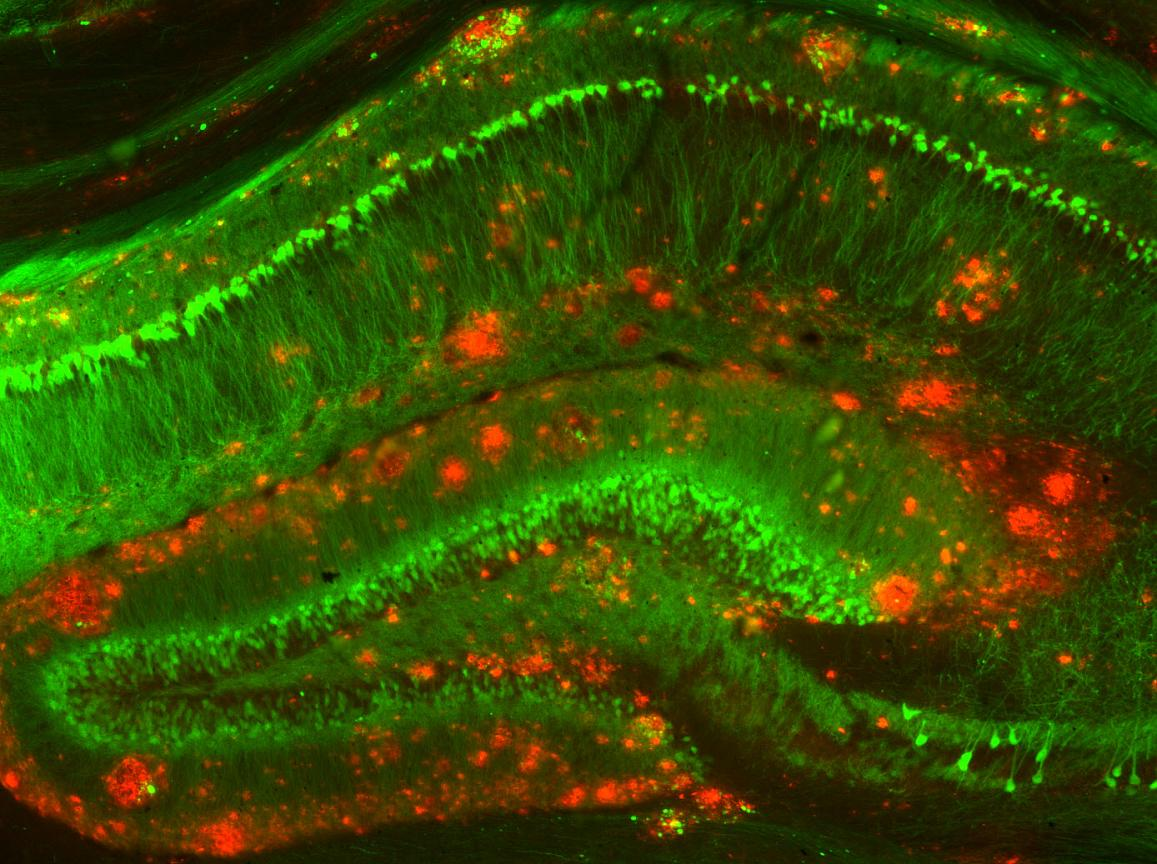
\includegraphics[width=0.61\textwidth]{static_figure/amyloid_aggregates.jpg}
\end{figure}

\footnotesize
Amyloid aggregates (red) around neurons (green). Strittmatter Laboratory, Yale University.

\end{frame}  

\begin{frame}{Amyloid proteins}

Functional amyloids:

\begin{itemize}
\item Pmel17,
\item RIP1 and RIP3,
\item acrosomal matrix proteins,
\item HET-s,
\item proteinaceous scaffolds of biofilms. 
\end{itemize}

\end{frame}  

  
\begin{frame}{Amyloid proteins}

Hot-spots:
\begin{itemize}
\item short (6-15 amino acids),
\item very high variability of amino acid composition,
\item initiate amyloid aggregation,
\item create specific "zipper-like" $\beta$-structures.
\end{itemize}

\begin{figure} 
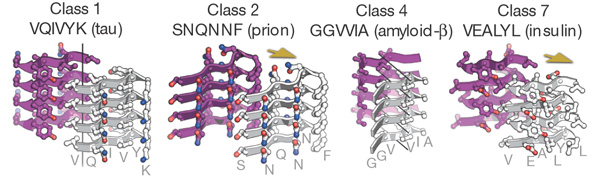
\includegraphics[width=0.9\textwidth]{static_figure/zipper_structure.jpg}
\end{figure}

\footnotesize\citet{sawaya_atomic_2007}
\end{frame}


\section{n-grams}

\begin{frame}
Computational analysis of biological sequences requires converting them to features understandable by machines.

The optimal conversion of information:
\begin{itemize}
\item loss-less,
\item concise.
\end{itemize}
\end{frame}  

\begin{frame}
n-grams (k-tuples, k-mers):
\begin{itemize}
\item subsequences (continuous or gapped) of $n$ residues,
\item considers the context of a specific residue.
\end{itemize}


% latex table generated in R 3.4.4 by xtable 1.8-2 package
% Tue May  1 08:46:19 2018
\begin{table}[ht]
\centering
\begin{tabular}{rlllll}
  \hline
 & P1 & P2 & P3 & P4 & P5 \\ 
  \hline
S1 & M & R & K & L & Y \\ 
   \hline
\end{tabular}
\end{table}



2-grams:
MR, RK, KL, LY

2-grams (gap 1):
M -- K, R -- L, K -- Y

3-grams:
MRK, RKL, KLY
\end{frame}  



\begin{frame}

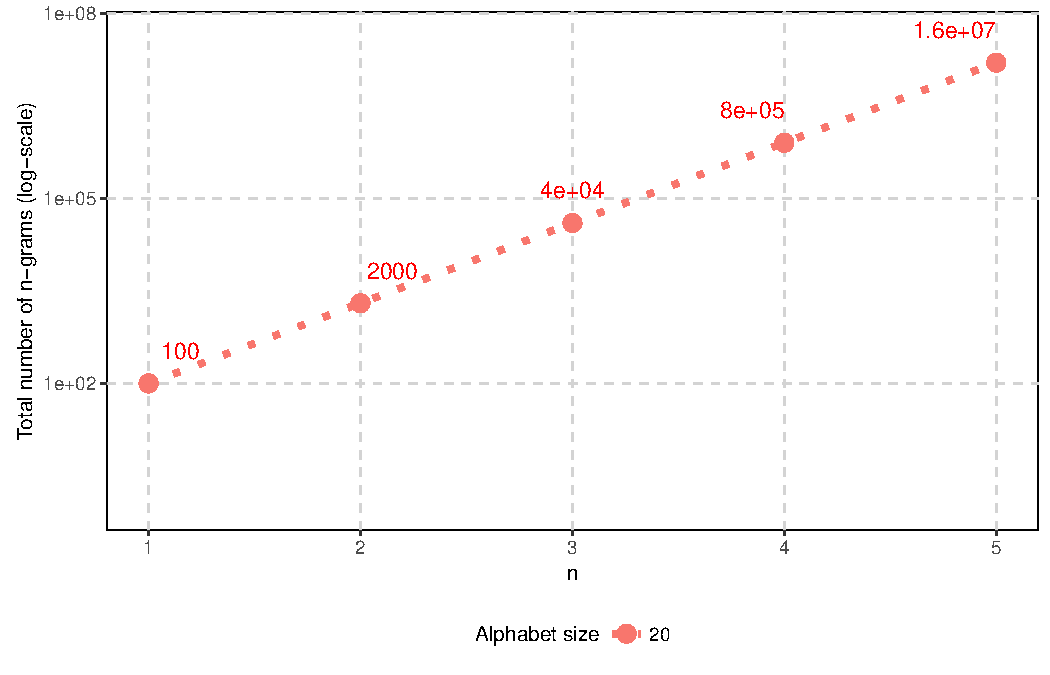
\includegraphics[width=\maxwidth]{figure/unnamed-chunk-5-1} 

Longer n-grams are more informative, but create larger feature spaces, which are hard to process and analyze.
\end{frame}

\begin{frame}{Permutation Tests}
  Informative n-grams are usually selected using permutation tests.

During a permutation test we shuffle randomly class labels and compute a defined statistic (e.g. information gain). Values of statistic for permuted data are compared with the value of statistic for original data.

$$
\textrm{p-value} = \frac{N_{T_P > T_R}}{N} $$

$N_{T_P > T_R}$: number of cases, where $T_P$ (permuted test statistic) has more extreme values than $T_R$ (test statistic for original data).

$N$: number of permutations.
  \end{frame}

\begin{frame}{QuiPT}  


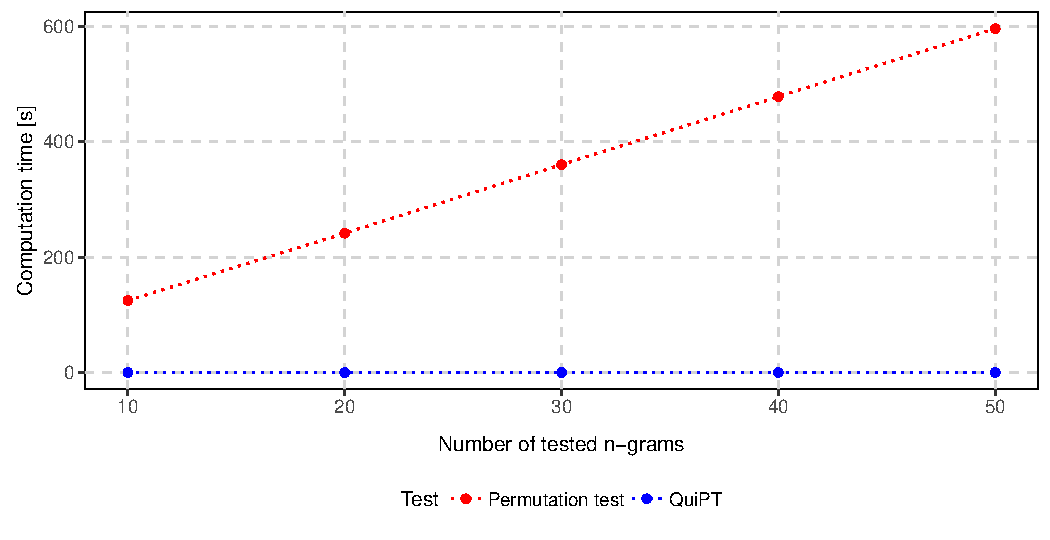
\includegraphics[width=\maxwidth]{figure/unnamed-chunk-6-1} 


QuiPT (available as a part of the \textbf{biogram} R package) is faster than classical permutation tests and returns exact p-values.
\end{frame}

\section{Simplified alphabets}

\begin{frame}
Simplified alphabets:
\begin{itemize}
\item are based on grouping amino acids with similar physicochemical properties,
\item ease computational analysis of a sequence~\citep{murphy_simplified_2000},
\item create more explicite models.
\end{itemize}
\end{frame}


\begin{frame}  
Two sequences that have drastically different amino acids composition may have very similar physicochemical properties.




Sequence I: 

\texttt{FKVWPDHGSG}

\medskip

Sequence II: 

\texttt{YMCIYRAQTN}

\end{frame}  


\begin{frame}

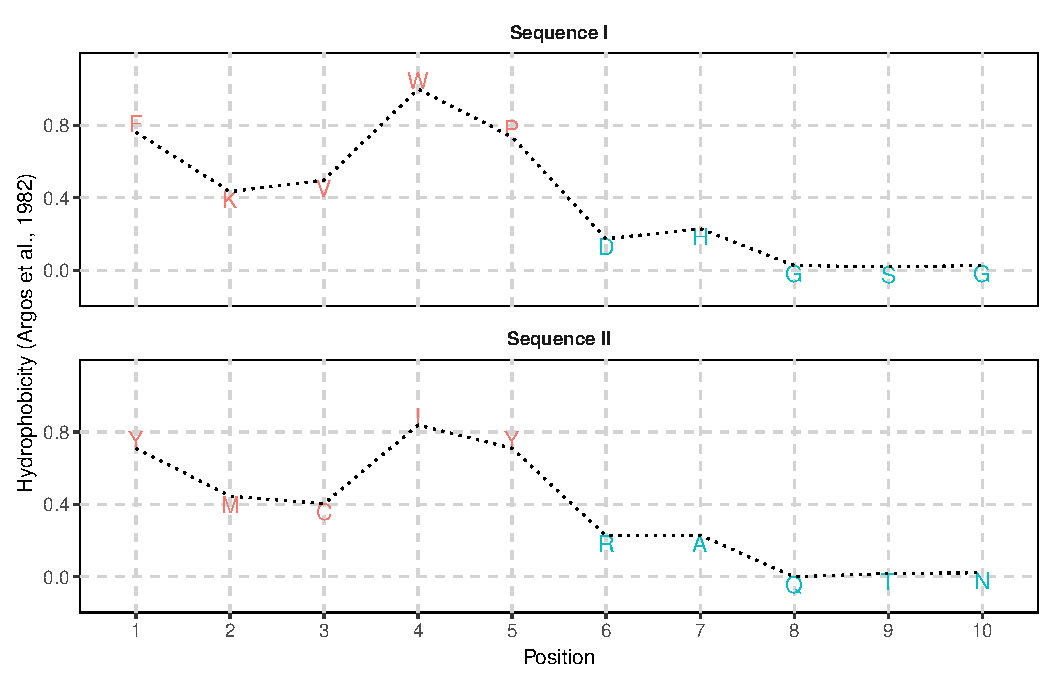
\includegraphics[width=\maxwidth]{figure/unnamed-chunk-8-1} 


\end{frame}  

\begin{frame}
\begin{table}
\begin{tabular}{cl}
\toprule
Subgroup & Amino acid \\ 
\midrule
  1 & C, I, L, K, M, F, P, W, Y, V \\ 
\rowcolor[gray]{0.85}  2 & A, D, E, G, H, N, Q, R, S, T \\ 
\bottomrule
\end{tabular}
\end{table}

\begin{columns}
\begin{column}{0.44\textwidth}
 
Sequence I: \texttt{FKVWPDHGSG} \textrightarrow

Sequence II: \texttt{YMCIYRAQTN} \textrightarrow

\end{column}
\begin{column}{0.5\textwidth}  %%<--- here

\texttt{1111122222}

\texttt{1111122222}
\end{column}
\end{columns}
\end{frame}  



\section{Prediction of amyloidogenicity}

\begin{frame}{Data}
AmyLoad: a database of amyloid fragments~\citep{WozniakAmyLoadwebsitededicated2015}.

\begin{itemize}
 \item 1465 fragments,
 \item 11915 residues,
 \item 421 aggregation-prone fragments,
 \item 4312 residues (36.19\%) in aggregation-prone fragments.
\end{itemize}

\end{frame}


\begin{frame}
Can we predict amyloid fragments using n-gram data?
\end{frame}


    \begin{frame}
\begin{figure} 
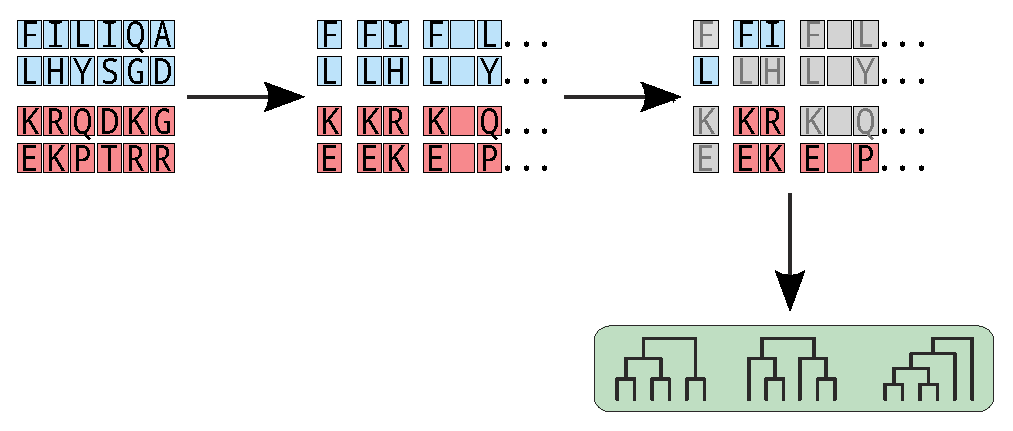
\includegraphics[width=0.95\textwidth]{static_figure/ngram1.eps}
\end{figure}
  \end{frame}

\begin{frame}{Cross-validation}
\begin{knitrout}
\definecolor{shadecolor}{rgb}{0.969, 0.969, 0.969}\color{fgcolor}

{\centering 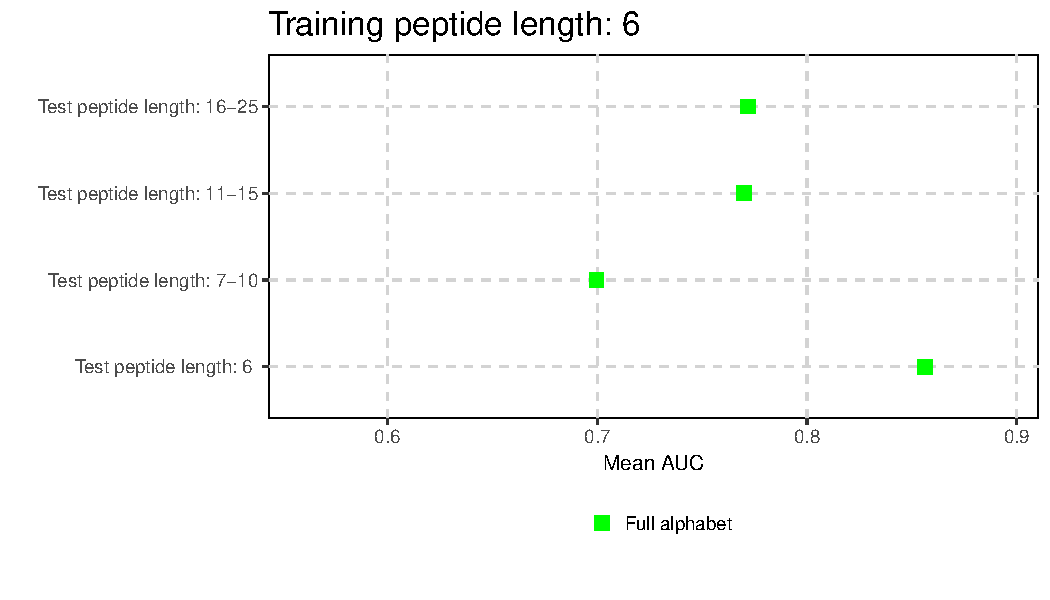
\includegraphics[width=\maxwidth]{figure/unnamed-chunk-9-1} 

}



\end{knitrout}
AUC (Area Under the Curve) measures the performance of a classifier (1 - classifier always properly recognizes amyloid proteins, 0 - classifier never properly recognizes amyloid proteins).

\end{frame}


\begin{frame}
  Does amyloidogenicity depend on the exact sequence of amino acids?
  \end{frame}

\begin{frame}{Standard simplified amino acid alphabets}
To date, several simplified amino acid alphabets have been proposed, which have been applied to (among others) protein folding and protein structure prediction~\citep{kosiol_new_2004, melo_accuracy_2006}.
  \end{frame}
  
    \begin{frame}{Standard simplified amino acid alphabets}
\begin{figure} 
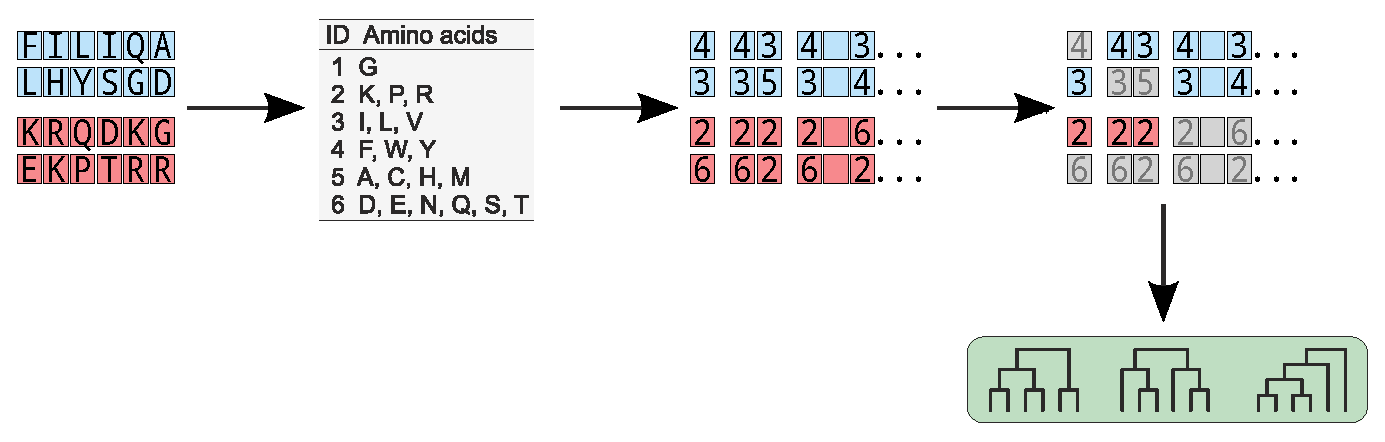
\includegraphics[width=0.95\textwidth]{static_figure/ngram2.eps}
\end{figure}


  \end{frame}


    \begin{frame}{Cross-validation}
\begin{knitrout}
\definecolor{shadecolor}{rgb}{0.969, 0.969, 0.969}\color{fgcolor}

{\centering 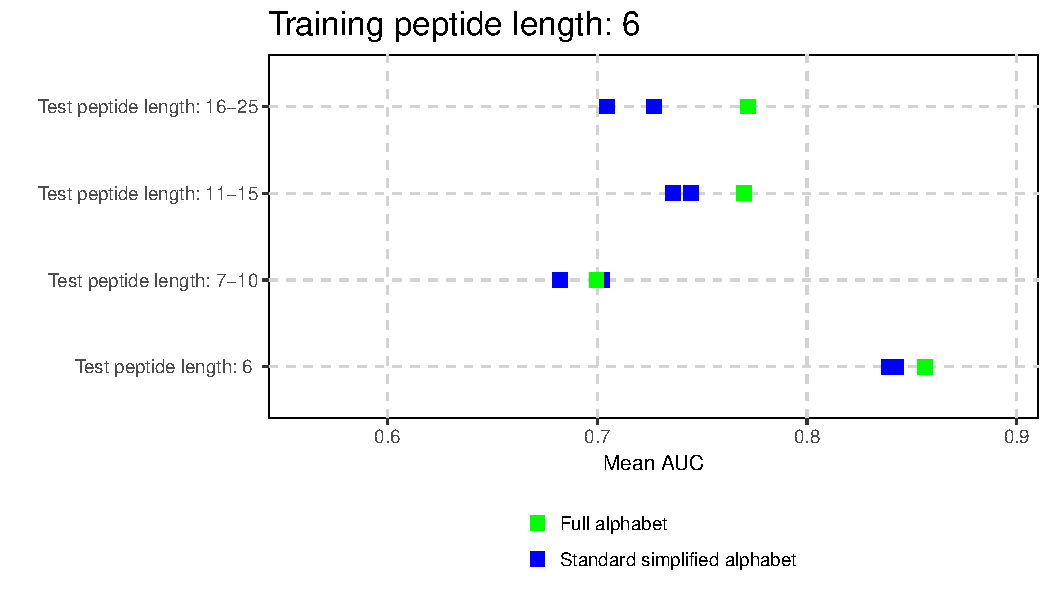
\includegraphics[width=\maxwidth]{figure/unnamed-chunk-10-1} 

}



\end{knitrout}

Standard simplified amino acid alphabets do not enhance discrimination between amyloidogenic and non-amyloidogenic proteins.
  
  \end{frame}


\begin{frame}{Novel simplified amino acid alphabets}

\begin{itemize}
\item 17 measures handpicked from AAIndex database: 
  \begin{itemize}
    \item size of residues, 
    \item hydrophobicity, 
    \item solvent surface area, 
    \item frequency in $\beta$-sheets,
    \item contactivity.
  \end{itemize}
  \item 524 284 amino acid simplified alphabets with different level of amino acid alphabet reduction (three to six amino acid groups).
  \end{itemize}

    \end{frame}
  
    \begin{frame}{Novel simplified amino acid alphabets}
\begin{figure} 
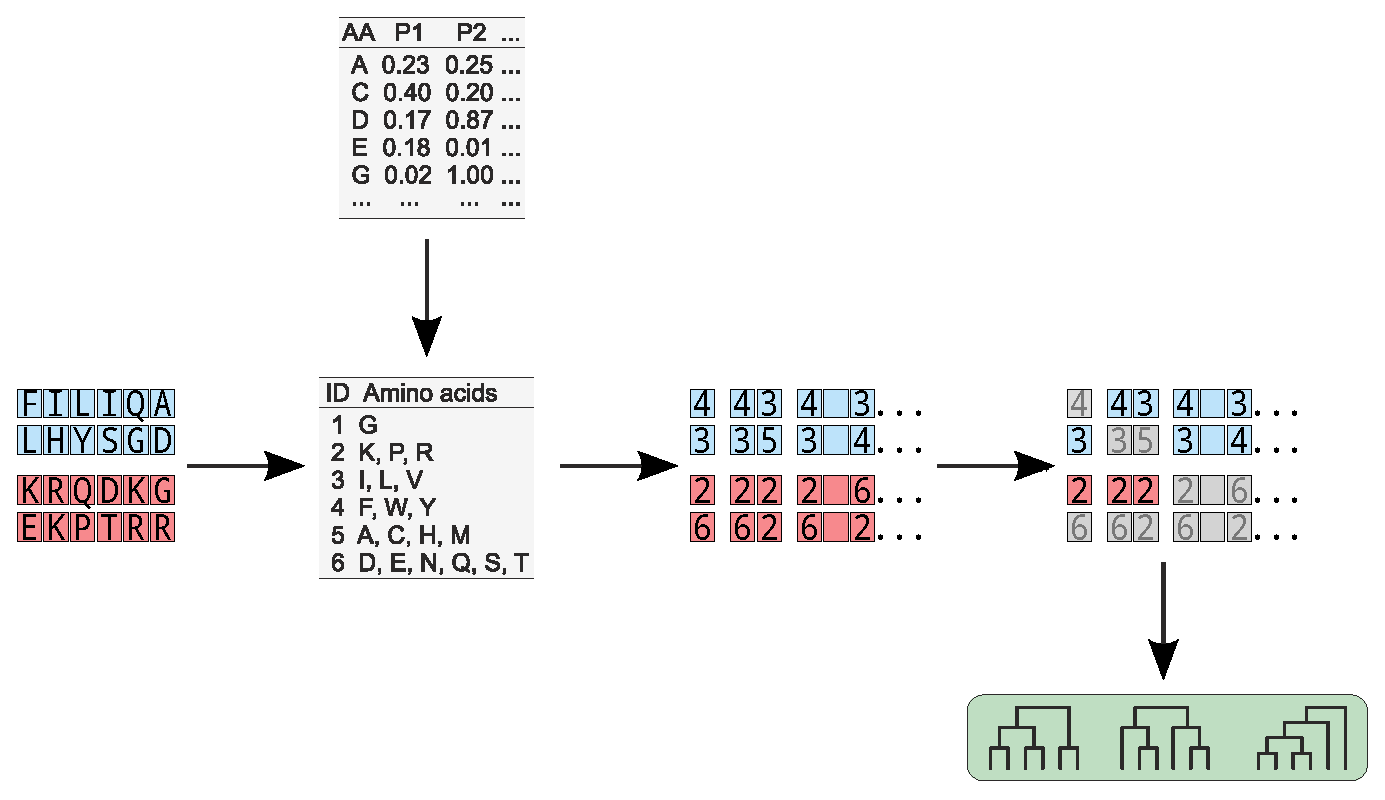
\includegraphics[width=0.95\textwidth]{static_figure/ngram3.eps}
\end{figure}
  \end{frame}



\begin{frame}{Cross-validation}
\begin{knitrout}
\definecolor{shadecolor}{rgb}{0.969, 0.969, 0.969}\color{fgcolor}

{\centering 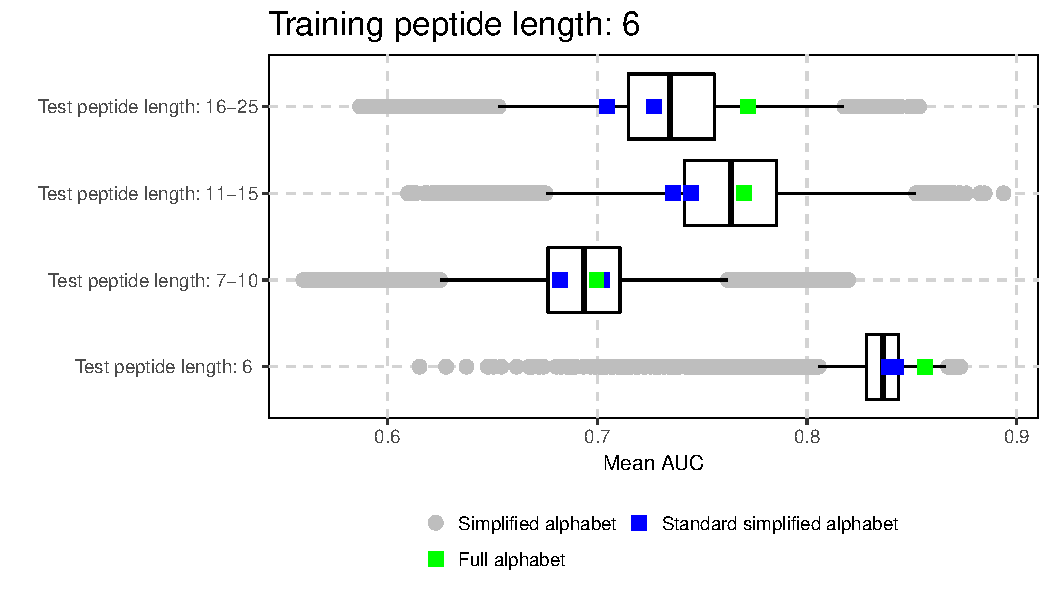
\includegraphics[width=\maxwidth]{figure/unnamed-chunk-11-1} 

}



\end{knitrout}
  \small
Hinges of boxes correspond to 
the 0.25 and 0.75 quartiles. The bar inside the box represents the median. The 
gray circles correspond to the simplified alphabets with the AUC outside the 0.95 
confidence interval.
  \end{frame}

\begin{frame}{Ranking alphabets}
\begin{knitrout}
\definecolor{shadecolor}{rgb}{0.969, 0.969, 0.969}\color{fgcolor}

{\centering 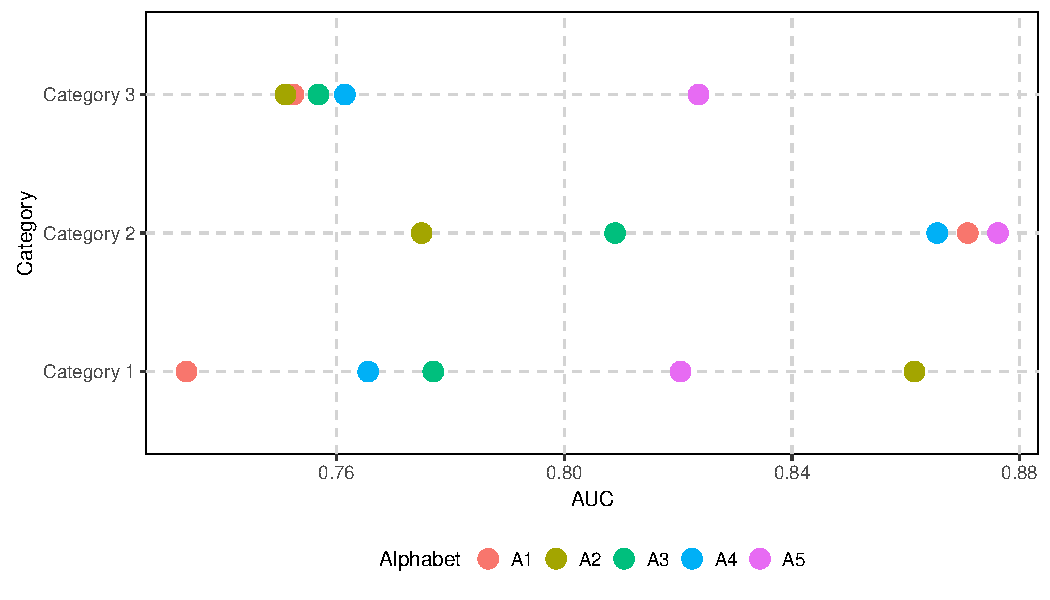
\includegraphics[width=\maxwidth]{figure/unnamed-chunk-12-1} 

}



\end{knitrout}
\end{frame}


\begin{frame}{Ranking alphabets}
\begin{knitrout}
\definecolor{shadecolor}{rgb}{0.969, 0.969, 0.969}\color{fgcolor}

{\centering 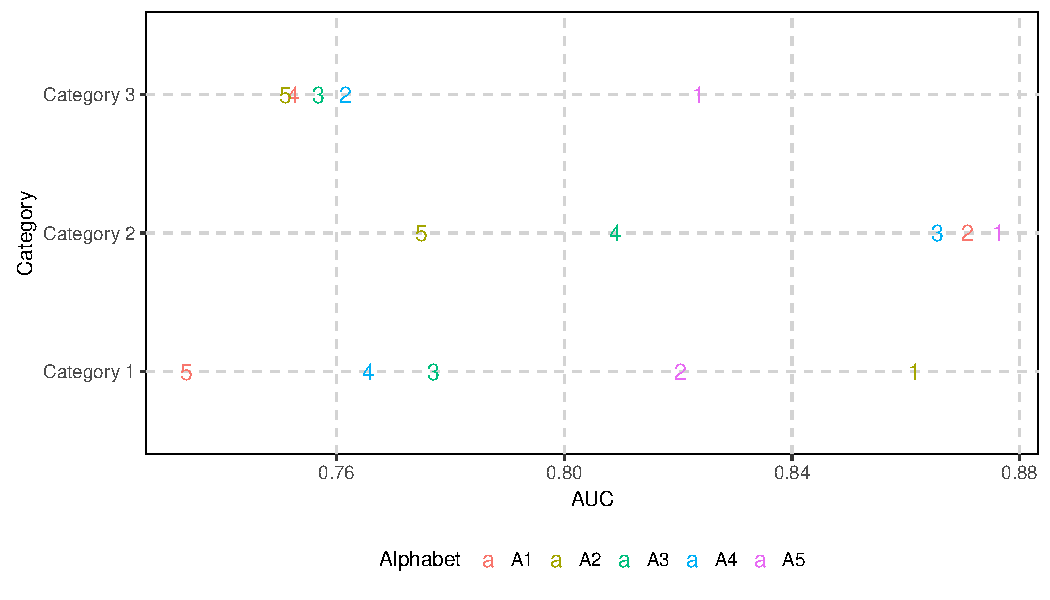
\includegraphics[width=\maxwidth]{figure/unnamed-chunk-13-1} 

}



\end{knitrout}
We rank alphabets separately in all length categories assuming the rank 1 for the best AUC, rank 2 for the second best AUC and so on.


\end{frame}

\begin{frame}{Ranking alphabets}
\begin{knitrout}
\definecolor{shadecolor}{rgb}{0.969, 0.969, 0.969}\color{fgcolor}

{\centering 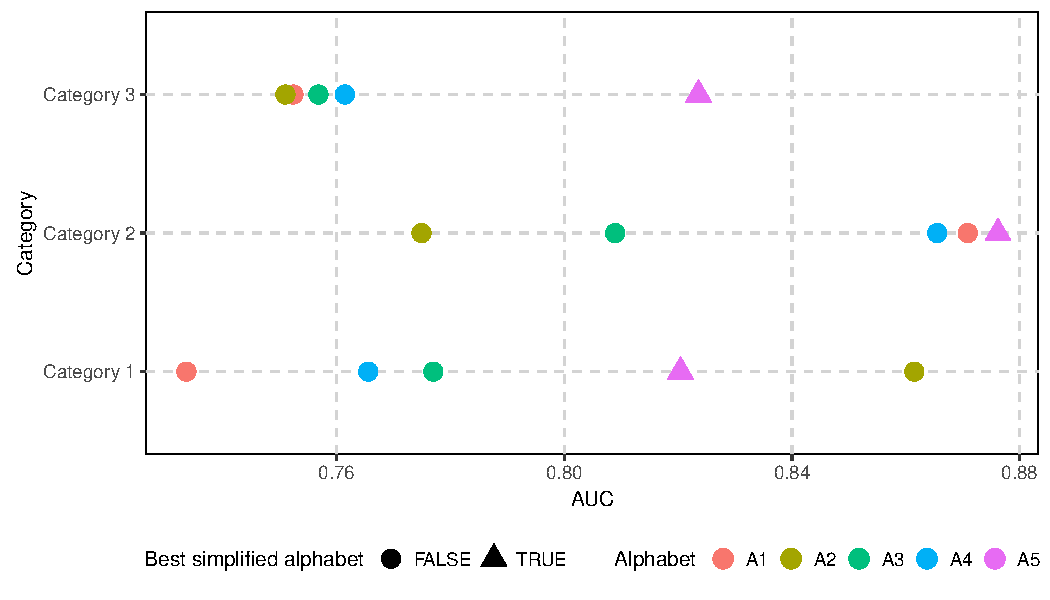
\includegraphics[width=\maxwidth]{figure/unnamed-chunk-14-1} 

}



\end{knitrout}
The best-performing alphabet has the lowest sum of ranks.  

\end{frame}
  
    \begin{frame}{The best-performing simplified alphabet}
\begin{knitrout}
\definecolor{shadecolor}{rgb}{0.969, 0.969, 0.969}\color{fgcolor}

{\centering 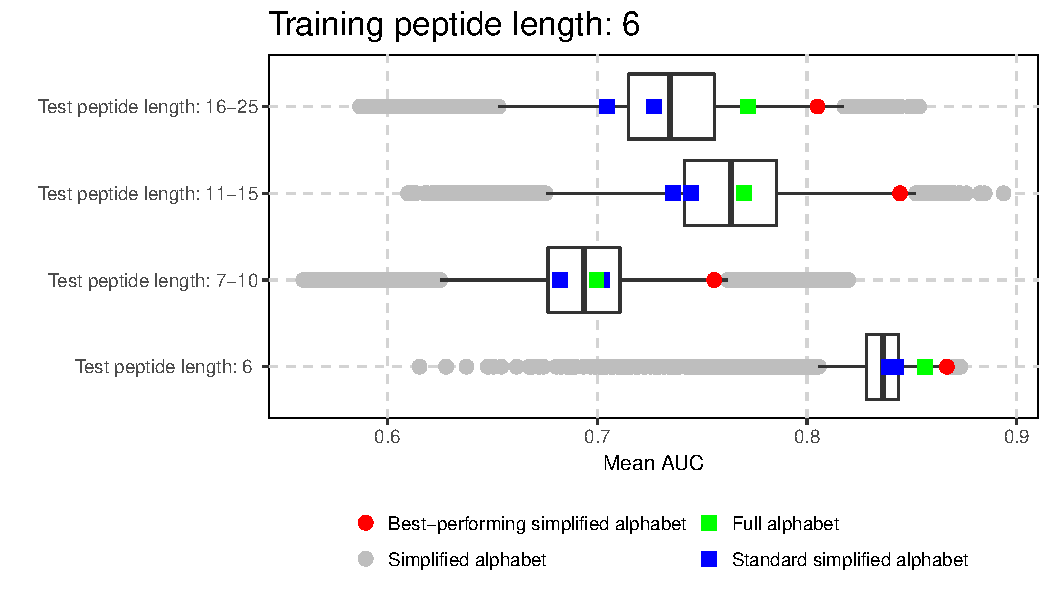
\includegraphics[width=\maxwidth]{figure/unnamed-chunk-15-1} 

}



\end{knitrout}
  \end{frame}

     \begin{frame}{The best-performing simplified alphabet}

   \begin{table}[ht]
\centering
\begin{tabular}{rl}
  \toprule
Subgroup ID & Amino acids \\ 
  \midrule
  1 & G \\ 
   \rowcolor[gray]{0.85}  2 & K, P, R \\ 
    3 & I, L, V \\ 
   \rowcolor[gray]{0.85}  4 & F, W, Y \\ 
    5 & A, C, H, M \\ 
   \rowcolor[gray]{0.85}  6 & D, E, N, Q, S, T \\ 
   \bottomrule
\end{tabular}
\end{table}
   
   \end{frame}

     \begin{frame}{The best-performing simplified alphabet}
   \begin{table}[ht]
\centering
\begin{tabular}{rl}
  \toprule
Subgroup ID & Amino acids \\ 
  \midrule
  1 & G \\ 
   \rowcolor[gray]{0.85}  2 & K, P, R \\ 
   \rowcolor{firebrick1} 3 & I, L, V \\ 
   \rowcolor{darkorange}  4 & F, W, Y \\ 
    5 & A, C, H, M \\ 
   \rowcolor[gray]{0.85}  6 & D, E, N, Q, S, T \\ 
   \bottomrule
\end{tabular}
\end{table}
   
Group 3 and 4 - hydrophobic amino acids.  
   \end{frame}
  
  
     \begin{frame}{The best-performing simplified alphabet}
   \begin{table}[ht]
\centering
\begin{tabular}{rl}
  \toprule
Subgroup ID & Amino acids \\ 
  \midrule
  1 & G \\ 
   \rowcolor{dodgerblue}  2 & K, P, R \\ 
    3 & I, L, V \\ 
   \rowcolor[gray]{0.85}  4 & F, W, Y \\ 
    5 & A, C, H, M \\ 
   \rowcolor[gray]{0.85}  6 & D, E, N, Q, S, T \\ 
   \bottomrule
\end{tabular}
\end{table}
   
Group 2 - charged breakers of $\beta$-structures.  
   
   \end{frame}  
   
\begin{frame}{Alphabet similarity and performance}
Is the best-performing simplified amino alphabet associated with amyloidogenicity?
\end{frame}

\begin{frame}{Similarity index}
\begin{knitrout}
\definecolor{shadecolor}{rgb}{0.969, 0.969, 0.969}\color{fgcolor}

{\centering 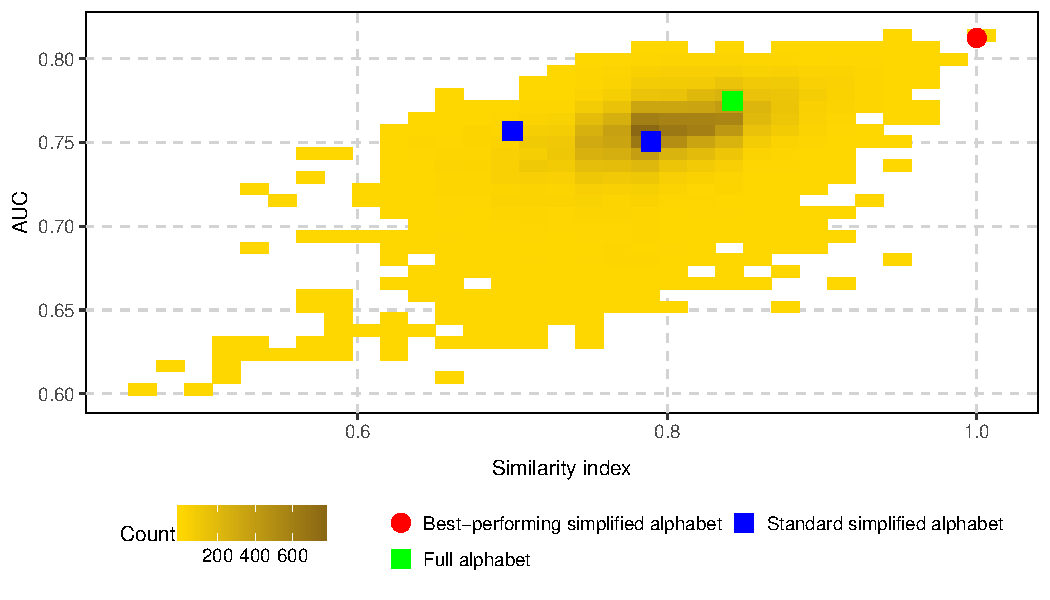
\includegraphics[width=\maxwidth]{figure/unnamed-chunk-17-1} 

}



\end{knitrout}
Similarity index~\citep{stephenson_unearthing_2013} measures the similarity between two simplified alphabets (1 - identical, 0 - totally dissimilar).
\end{frame}



\begin{frame}{Similarity index}
\begin{knitrout}
\definecolor{shadecolor}{rgb}{0.969, 0.969, 0.969}\color{fgcolor}

{\centering 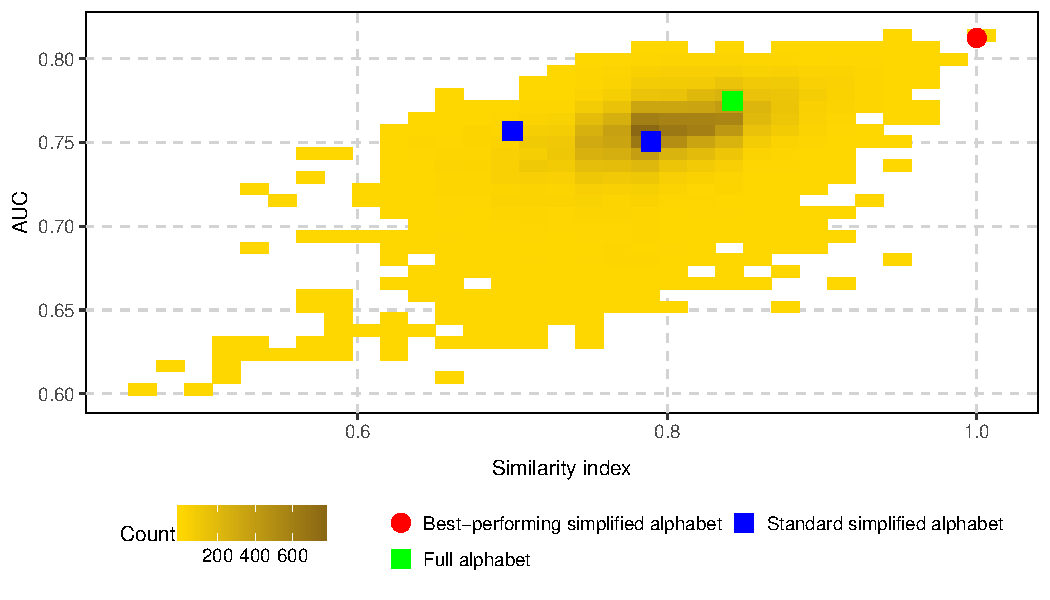
\includegraphics[width=\maxwidth]{figure/unnamed-chunk-18-1} 

}



\end{knitrout}
The color of a square is proportional to the number of simplified alphabets in its area.
\end{frame}

\begin{frame}{Similarity index}
\begin{knitrout}
\definecolor{shadecolor}{rgb}{0.969, 0.969, 0.969}\color{fgcolor}

{\centering 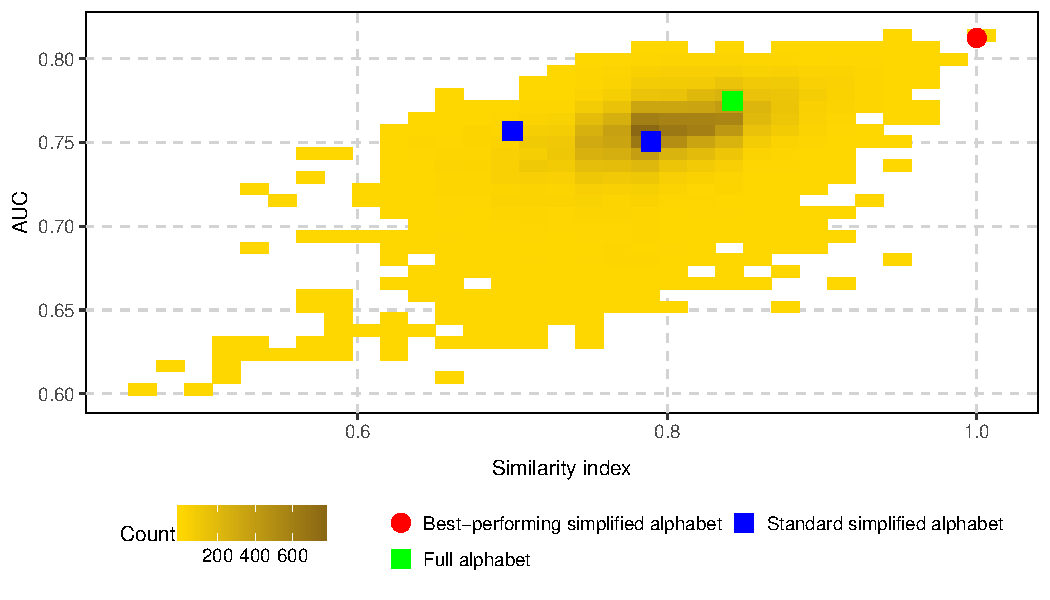
\includegraphics[width=\maxwidth]{figure/unnamed-chunk-19-1} 

}



\end{knitrout}
The correlation between mean AUC and similarity index is significant ($\textrm{p-value} \leq 2.2^{-16}$; $\rho = 0.51$).
\end{frame}
   
\begin{frame}{}
Are informative n-grams found by QuiPT associated with amyloidogenicity?
\end{frame}


\begin{frame}{Informative n-grams}
\begin{figure} 
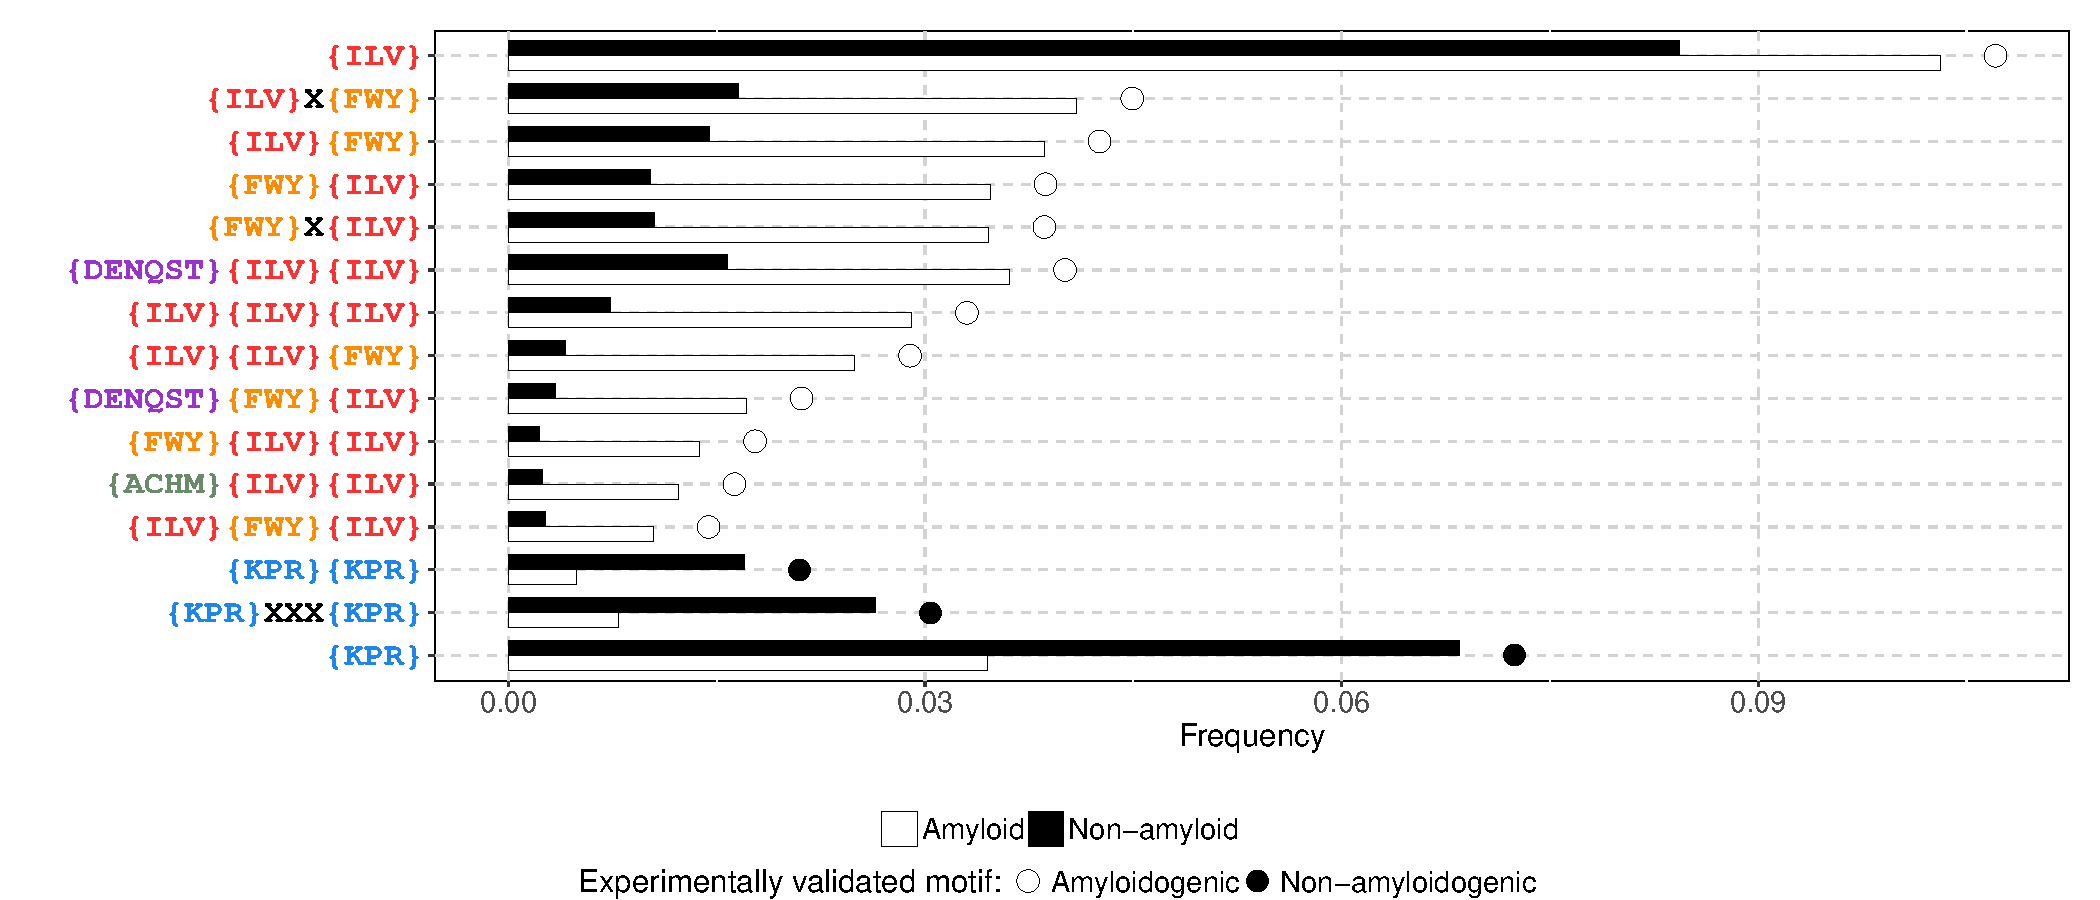
\includegraphics[width=0.99\textwidth]{static_figure/ngrams.pdf}
\end{figure}

Out of 65 the most informative n-grams, 15 (23\%) were also found in the motifs validated experimentally~\citep{paz_sequence_2004}.
\end{frame}


\begin{frame}{Benchmark results}

\begin{table}[ht]
\centering

\begin{tabular}{ccccc}
  \toprule
Classifier & AUC & MCC \\ 
  \midrule
AmyloGram & \textbf{0.8972} & \textbf{0.6307} \\ 
  \rowcolor{white}PASTA 2.0 \citep{walsh_pasta_2014} & 0.8550 & 0.4291  \\ 
   FoldAmyloid \citep{garbuzynskiy_foldamyloid:_2010} & 0.7351 & 0.4526  \\ 
  \rowcolor{white}APPNN \citep{familia_prediction_2015} & 0.8343 & 0.5823  \\ 
   \bottomrule
\end{tabular}
\end{table}

The predictor based on the best-performing alphabet, called AmyloGram, was benchmarked against the most popular tools for the detection of amyloid peptides using an external data set \textit{pep424}.

\footnotesize

\end{frame}

\begin{frame}{Benchmark results}

\begin{table}[ht]
\centering

\begin{tabular}{ccccc}
  \toprule
Classifier & AUC & MCC \\ 
  \midrule
AmyloGram & \textbf{0.8972} & \textbf{0.6307} \\ 
  \rowcolor{white}PASTA 2.0 \citep{walsh_pasta_2014} & 0.8550 & 0.4291  \\ 
   FoldAmyloid \citep{garbuzynskiy_foldamyloid:_2010} & 0.7351 & 0.4526  \\ 
  \rowcolor{white}APPNN \citep{familia_prediction_2015} & 0.8343 & 0.5823  \\ 
   \bottomrule
\end{tabular}
\end{table}

MCC (Matthew's Correlation Coefficient) measures the performance of a classifier (1 - classifier always properly recognizes amyloid proteins, -1 - classifier never properly recognizes amyloid proteins).

\footnotesize

\end{frame}



\begin{frame}{Experimental validation}
\begin{figure} 
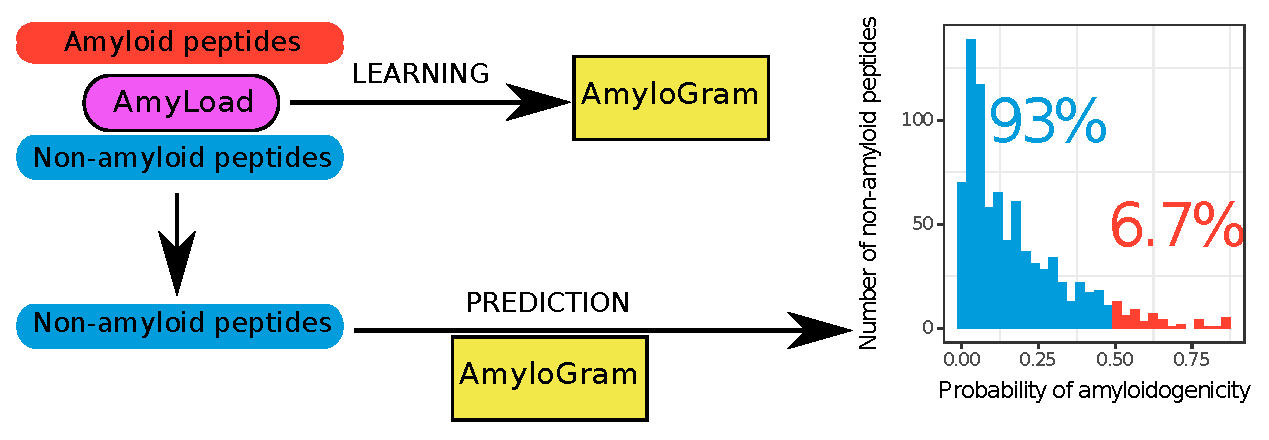
\includegraphics[width=0.95\textwidth]{static_figure/diagram1.eps}
\end{figure}
\end{frame}

\begin{frame}{Experimental validation}
\begin{figure} 
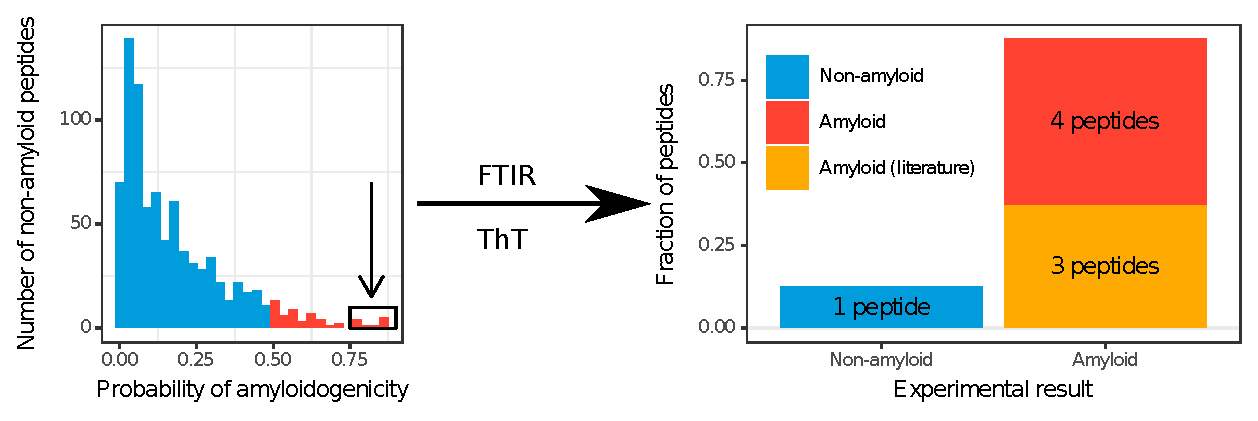
\includegraphics[width=0.95\textwidth]{static_figure/diagram2.eps}
\end{figure}
\end{frame}


\section{Perspectives and summary}

\begin{frame}{Perspectives}
Improved prediction of amyloid proteins:
\begin{itemize}
\item hot-spots in the context of the whole protein,
\item association of amino acid motifs and amyloidogenicity.
\end{itemize}

Goal: proteome-wide \textit{in silico} detection of amyloid proteins.

Limitations: very few proteins with known aggregation-prone regions.

\textbf{AmyPro}: a database of amyloid proteins.

\begin{itemize}
 \item 143 proteins,
 \item 40719 residues,
 \item 174 aggregation-prone regions,
 \item 5645 residues (13.86\%) in aggregation-prone regions.
\end{itemize}

\end{frame}  


\begin{frame}{Perspectives}
Seeding and cross-seeding: families of hot spots and relaxed seeding specificity.
\begin{itemize}
\item CsgA, CsgB, $\alpha$-synuclein,
\item FapC and FapB.
\end{itemize}

Goal: identification of potential cross-seeding proteins in human microbiome.
\end{frame}  

\begin{frame}{Perspectives}
Hot-spot specific inhibitors of amyloidogenicity (CsgC, TTR).

Goal: co-evolution of amyloid and its inhibitor.
\end{frame}  

\begin{frame}{Availability}
Software packages:
\begin{itemize}
\item \textbf{biogram}: \url{https://cran.r-project.org/package=biogram}.
\item \textbf{AmyloGram}: \url{https://cran.r-project.org/package=AmyloGram}.
\end{itemize}

Web servers:
\begin{itemize}
\item \textbf{AmyloGram}: \url{http://www.smorfland.uni.wroc.pl/shiny/AmyloGram/}.
\end{itemize}
\end{frame}  

\begin{frame}{Summary}
\begin{enumerate}
\item Created a new, accurate predictor of amyloids~\citep{BurdukiewiczAmyloidogenicmotifsrevealed2017}.
\item Found a set of amino acid motifs associated with the amyloidogenic properties or the lack of them.
\item Found a simplified alphabet suitable for prediction of amyloid proteins.
\end{enumerate}
\end{frame}  

\begin{frame}{Acknowledgments}
Mentors:
\begin{itemize}
\item \textbf{Paweł Mackiewicz (University of Wrocław)}.
\item Lars Kaderali (University of Greifswald).
\item Małgorzata Kotulska (Wrocław University of Science and Technology).
\item Henrik Nielsen (Technical University of Denmark).
\item Stefan Rödiger (Brandenburg University of Technology Cottbus-Senftenberg).
\item Vytauas Smirnovas (University of Vilnus). 
\end{itemize}
\end{frame}


\begin{frame}{Acknowledgments}
Peers:
\begin{itemize}
\item Agata Błaszczyńska (Wrocław University of Science and Technology).
\item Anna Duda-Madej (Wrocław Medical University).
\item Marlena G\k{a}sior-Głogowska (Wrocław University of Science and Technology).
\item Chris Lauber (Technical University Dresden).
\item Natalia Niedzielska (Wrocław University of Science and Technology).
\item Piotr Sobczyk (Wrocław University of Science and Technology).
\end{itemize}

\end{frame}

\begin{frame}{Acknowledgments}
Funding:
\begin{itemize}
\item National Science Center (grants 2015/17/N/NZ2/01845 and 2017/24/T/NZ2/00003).
\item COST ACTION CA15110 (Harmonising standardisation strategies to increase efficiency and competitiveness of European life-science research).
\item KNOW Wrocław Center for Biotechnology.
\end{itemize}

\end{frame}

\begin{frame}{Summary}
\begin{enumerate}
\item Created AmyloGram, a new, accurate predictor of amyloids~\citep{BurdukiewiczAmyloidogenicmotifsrevealed2017}.
\item Found a set of amino acid motifs associated with the amyloidogenic properties or the lack of them.
\item Found a simplified alphabet suitable for prediction of amyloid proteins.
\end{enumerate}

\textbf{AmyloGram}: \url{http://www.smorfland.uni.wroc.pl/shiny/AmyloGram/}.

\end{frame}  


\begin{frame}[allowframebreaks]
        \frametitle{References}
  \bibliographystyle{apalike}
  \bibliography{references}
\end{frame}  


\end{document}
